% Analisi dei requisiti

\chapter{Analisi dei requisiti}\label{chap:requirements}

\section{Attori coinvolti}
Durante l'attività di analisi dei requisiti sono stati individuati quattro 
attori capaci di interagire attivamente con l'applicazione \emph{Teamwork}. 
Di questi tre sono attori principali, mentre uno è un attore secondario.
\subsection{Attori principali}
\subsubsection{Utente Zimbra}
L'applicazione è destinata solamente agli utenti \emph{Zimbra}. Ciò implica che
si possa accedere alle funzionalità di \emph{Teamwork} esclusivamente se si è
già in possesso di un'email \emph{Zimbra} gestita dai loro \emph{server}. Tale
scenario è rappresentato dall'attore più generico.
\subsubsection{Utente OpenChat}
Un utente \emph{OpenChat}, specializzazione dell'utente \emph{Zimbra}, rappresenta un utente che utilizza un'istanza di Zimbra con la \emph{zimlet OpenChat} installata. Quest'ultima permette di chattare con gli utenti \emph{Zimbra} dello stesso server.

\subsubsection{Utente Teamwork web}
Un utente \emph{Teamwork} web, specializzazione dell'utente \emph{OpenChat}, rappresenta 
un utente che, oltre ad utilizzare un'istanza di \emph{Zimbra} con la \emph{zimlet OpenChat}, 
ha installato anche la \emph{zimlet Teamwork}, applicazione di chat potenziata rispetto 
alla prima e disponibile solo per la \emph{suite Zextras}.

\subsection{Attori secondari}
\subsubsection{Server Zimbra}
Un server \emph{Zimbra} è un'istanziazione della suite di prodotti \emph{Zimbra} e, in caso, 
dei prodotti \emph{Zextras}. Tramite esso è possibile accedere a tutti i dati del profilo \emph{Zimbra} 
così da mantenerli sincronizzati tra le varie sessioni in uso.

\section{Casi d'uso principali}
Considerando l'obbiettivo del progetto (sez. \ref{sec:intaz}) e il metodo di 
lavoro utilizzato (sez. \ref{sec:pianificazione}), i casi d'uso (come i
requisiti funzionali) sono stati sviluppati e modificati durante tutto il corso
del progetto.
Per l'identificazione dei requisiti funzionali sono stati delineati  i casi d'uso principali tramite le richieste dell'azienda e quelli  di alto livello, in modo da poter dare una visione d’insieme più precisa del prodotto sviluppato. \\
La Figura~\ref{fig:ucg} rappresenta il diagramma dei casi d'uso principali.
\begin{figure}[H] 
	\centering
	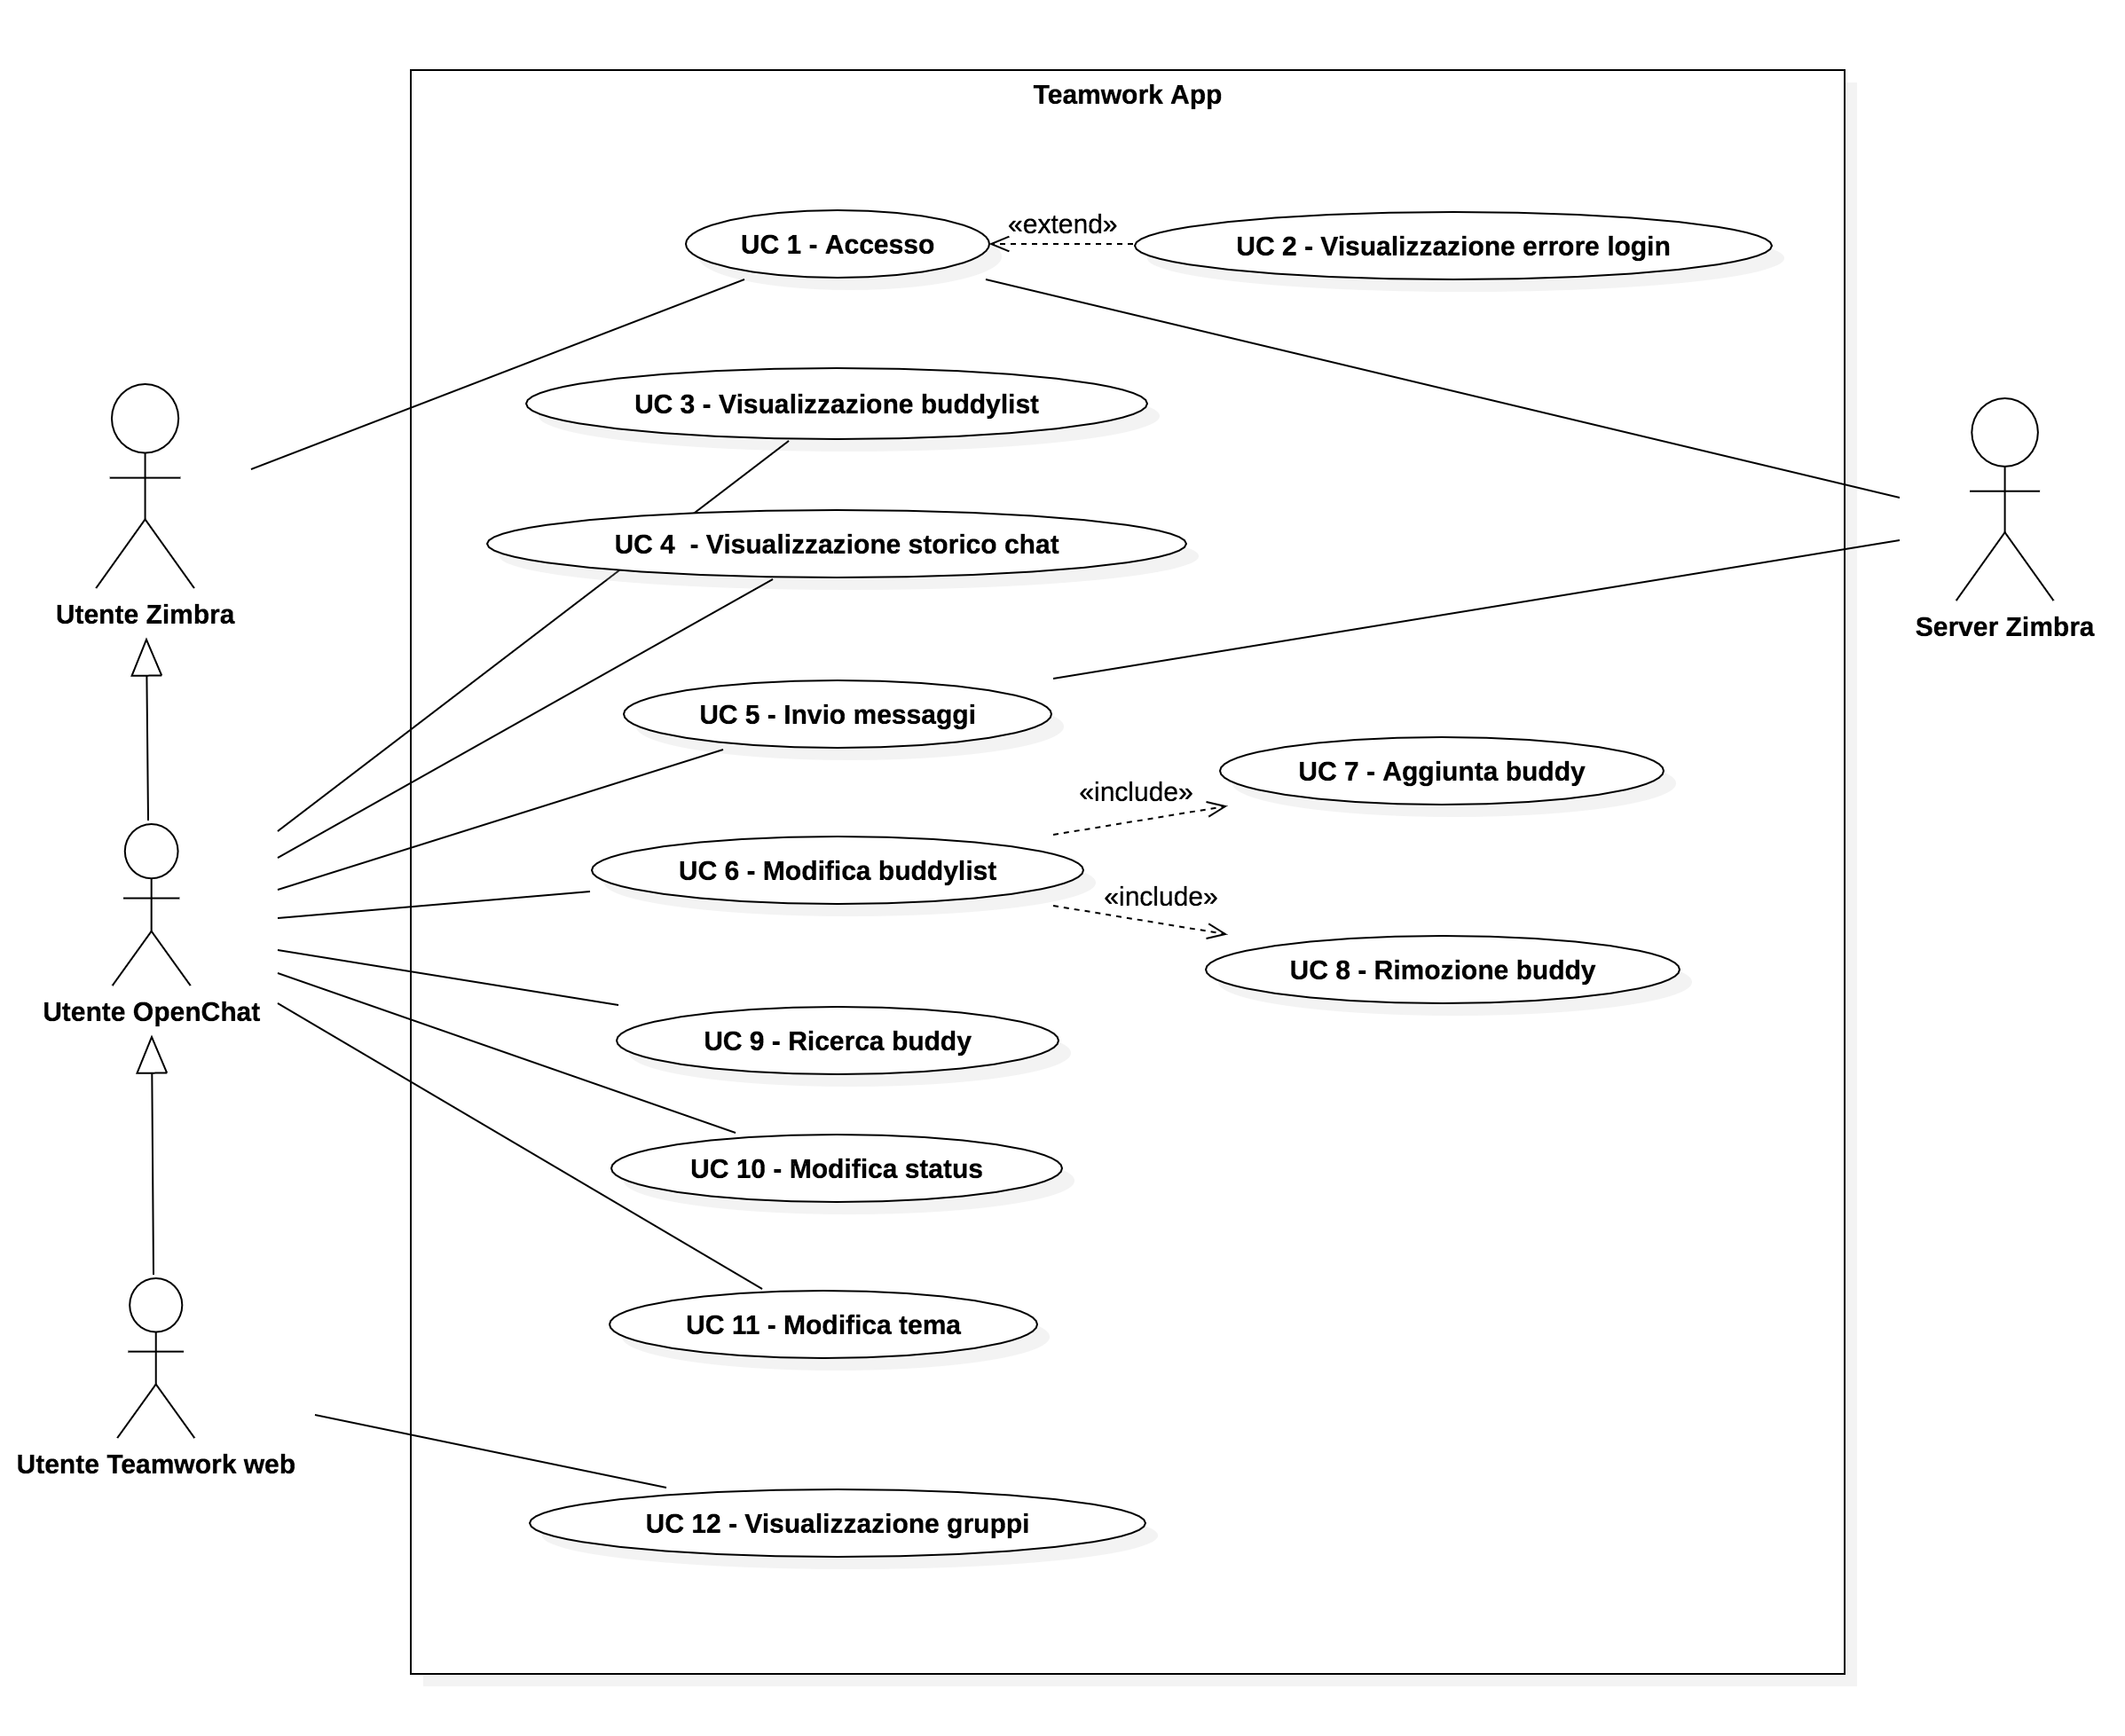
\includegraphics[scale=0.17]{UC/UCG}
	\caption{Casi d'uso principali}
	\label{fig:ucg}
\end{figure}
In appendice \ref{A1} è possibile trovare una descrizione esaustiva dei casi
d'uso studiati.

\section{Requisiti}
Ogni requisito di seguito riportato è identificato da un codice, ed è
rappresentato nel seguente modo:
$$ \textbf{R \{importanza\}\{tipo\}\{numero\_vincolo\} } $$

\begin{itemize}
	\item "R" è prefisso di tutti i codici dei requisiti;
	\item Il primo valore rappresenta l'importanza: \textbf{0} se il requisito è obbligatorio, \textbf{1} se è desiderabile, \textbf{2} per gli opzionali;
	\item Il terzo valore indica il tipo: \textbf{F} per i requisiti funzionali, \textbf{Q} per quelli di qualità, \textbf{P} se prestazionale, \textbf{V} se di vincolo;
	\item L'ultimo numero indica il numero del vincolo. La struttura numerica di quest'ultimo rispetta le stesse regole dei Casi D'Uso.
\end{itemize}

\subsection{Principali requisiti funzionali}
\begin{longtable}{|C{3cm}| C{10cm}|}
	\hline
	\textbf{Id Requisito} & \textbf{Descrizione}\\
	\hline
	\endhead
	R0F1 & L'utente Zimbra deve poter effettuare l'accesso inserendo inserendo l'email e la password con cui è registrato al server Zimbra.  \\ \hline 
	R0F1.1 & L'utente Zimbra può inserire la propria mail. \\ \hline 
	R0F1.2 & L'utente Zimbra  può inserire la propria password dell'account Zimbra.\\ \hline 
	R0F2 & Il sistema deve mostrare un messaggio di errore in caso di inserimento dei dati errati o mancanti.  \\ \hline 
	R0F3 & L'utente OpenChat deve poter vedere la propria buddylist una volta effettuato l'accesso all'applicazione. \\ \hline 
	R1F3.1 & L'utente OpenChat deve poter vedere per ogni buddy della sua buddylist una card contenente dei dettagli relativi al buddy. \\ \hline 
	R1F3.1.1 & L'utente OpenChat deve poter vedere per ogni buddy della sua buddylist il nickname corrispondente. \\ \hline 
	R1F3.1.2 & L'utente OpenChat deve poter vedere per ogni buddy della sua buddylist l'immagine profilo corrispondente. \\ \hline 
	R1F3.1.3 & L'utente OpenChat deve poter vedere per ogni buddy della sua buddylist lo status in cui si trova. \\ \hline 
	R1F3.1.4 & L'utente OpenChat deve poter vedere per ogni buddy della sua buddylist la data dell'ultimo messaggio scambiato con tale utente. \\ \hline 
	R1F3.1.5 & L'utente OpenChat deve poter vedere per ogni buddy della sua buddylist il numero dei messaggi ricevuti non ancora letti. \\ \hline 
	R0F4 & L'utente OpenChat deve poter vedere per ogni buddy della sua buddylist lo storico delle conversazioni avute. \\ \hline 
	R0F4.1 & L'utente OpenChat deve poter vedere per ogni buddy della sua buddylist i messaggi ricevuti. \\ \hline 
	R0F4.2 & L'utente OpenChat deve poter vedere per ogni buddy della sua buddylist i messaggi inviatogli. \\ \hline 
	R0F5 & L'utente OpenChat deve poter inviare messaggi ad ogni buddy della sua buddylist.\\ \hline 
	R1F6 & L'utente OpenChat deve poter modificare la sua buddylist.\\ \hline 
	R1F7 & L'utente OpenChat deve poter aggiungere un nuovo buddy alla sua buddylist conoscendone l'e-mail.\\ \hline 
	R1F8 & L'utente OpenChat deve poter rimuovere un buddy dalla sua buddylist così che non possa più contattarlo.\\ \hline 
	R2F9 & L'utente OpenChat deve poter ricercare i buddy tra quelli presenti nella sua buddylist in base a dei caratteri.\\ \hline 
	R1F10 & L'utente OpenChat deve poter modificare il proprio status con cui viene visualizzato dagli altri utenti..\\ \hline 
	R2F11 & L'utente OpenChat deve poter modificare il tema dei colori dell'applicazione.\\ \hline 
	R1F12 & L'utente OpenChat deve poter visualizzare i gruppi di cui fa parte.\\ \hline 
	
	\caption{Requisiti funzionali}
	\label{tabella:req}
\end{longtable}

\subsection{Requisiti di vincolo}
\begin{longtable}{|C{3cm}|C{10cm}|}
	\hline
	\textbf{Id Requisito} & \textbf{Descrizione}\\
	\hline
	\endhead
	R0V1 & L'applicazione deve essere sviluppata in React Native. \\ \hline 
	R0V2 & L'applicazione deve essere disponibile per iOS.  \\ \hline 
	R0V3 & L'applicazione deve essere disponibile per Android.  \\ \hline 
	R0V4 & Lo sviluppo dell'applicazione deve prevedere l'SDK Expo. \\ \hline 
	R1V5 & Il codice dell'applicazione può essere scritto in TypeScript.  \\ \hline 
	\caption{Requisiti di vincolo}
	\label{tabella:reqV}
\end{longtable}

\subsection{Requisiti di qualità}
\begin{longtable}{|C{3cm}|C{10cm}|}
	\hline
	\textbf{Id Requisito} & \textbf{Descrizione}\\
	\hline
	\endhead
	R0Q1 & L'applicazione deve sincronizzare i dati con quelli delle altre sessioni aperte.  \\ \hline 
	R0Q2 & L'interfaccia grafica deve rispettare le linee guida fornite dall'azienda.  \\ \hline 
	R0Q3 & Deve essere disponibile una documentazione per gli sviluppi futuri.  \\ \hline 
	R1Q4 & L'esperienza utente deve essere allineata con la soluzione già disponibile in ambiente web \\ \hline 
	\caption{Requisiti di qualità}
	\label{tabella:reqQ}
\end{longtable}

